\documentclass[10pt]{beamer}
%\usetheme{Madrid}
%\newlength{\pageheight}
%\setlength{\pageheight}{10cm}
%\usepackage{handoutWithNotes}
%\pgfpagesuselayout{2 on 1 with notes landscape}[a4paper,border shrink=5mm]

\usepackage[utf8]{inputenc}
\usepackage{dirtytalk}

\definecolor{darkgreen}{rgb}{0.0, 0.5, 0.0}

\usepackage{pgf}
\usepackage{tikz}
\usetikzlibrary{arrows,automata}
\beamertemplatenavigationsymbolsempty

\addtobeamertemplate{title page}{\includegraphics[scale=.05]{{University_of_Pittsburgh_seal.png}} \hfill 
\includegraphics[scale=.3]{fabstracts2.png}}{}


%\titlegraphic{
%    \begin{tikzpicture}[overlay, remember picture]
%\node[at=(current page.north), anchor=north] {%
%    
\includegraphics[width=0.2\textwidth]{University_of_Pittsburgh_seal.png}
%    
\includegraphics[width=0.35\textwidth]{fabstracts.png}
%        };
%    \end{tikzpicture}
%}

\title{Project Proposal: Creating a Database of Definitions From Large Mathematical Corpora}
\subtitle{A comprehensive dictionary of all mathematical lexicon}
\author{Luis Berlioz\\
\texttt{lab232@pitt.edu}}
\institute{University of Pittsburgh}

% Explain _inline_math_ better
% Explain all the acronyms BIO, SVC, nltk
% Credit Bruce Miller
% Keep one term for everything e.g. latex equation

\begin{document}
\begin{frame}
\titlepage
\end{frame}
\section{Objectives}

%%%%FRAME
\begin{frame}{Objectives and Outline}
    \begin{block}{Objective}
    \textit{Create a machine learning system that can find the definitions and the terms being defined in large collections of mathematical texts. }
    \end{block}


    The problem is broken down into two parts:
\begin{description}
    \item[The Classifier:] Tells if a given paragraph is a definition or not
    \item[A Named Entity Recognition system:] given a definition, returns the term that is being defined (definiendum).
%\item \say{\textit{When one starts to delve into the language of mathematics, one encounters
%        a phenomenon that is much more remarkable than the use of symbols. Mathematical language \emph{expands} as more mathematics is encountered.}} Mohan Ganisalengam.
%    \item \say{\textit{...the proof of [Stokes’] theorem is, in the mathematician’s sense, an utter triviality — a straight-forward calculation. On the other hand, even the statement of this triviality cannot be understood without a horde of definitions... There are good reasons why the theorems should all be easy and the definitions hard...}}  Michael Spivak.
\end{description}
For each part I will describe how to:
        \begin{itemize}
                \item Get and process the relevant  data.
                \item Train and take a look at the results.
        \end{itemize}
\end{frame}

\section{Data Pipeline}
%%%%FRAME
\begin{frame}{arXiv Website Bulk Download}
    \framesubtitle{All the \LaTeX{} source files can be downloaded from an Amazon S3 bucket}
    \begin{columns}[T]
        \begin{column}{0.5\textwidth}
    
\includegraphics[width=\textwidth]{bulk_download.png} 
        \end{column}
        \begin{column}{0.6\textwidth}
            \begin{itemize}
                \item About 885 Gigabytes of .tar files.
                \item Each .tar file is about 500 Megabytes.
                \item Download without affecting the website's traffic.
                \item \LaTeX{} source is converted to a more structured format.
            \end{itemize}
        \end{column}
    \end{columns}
\end{frame}

%%%%FRAME
\begin{frame}{LaTeXML}
    \framesubtitle{Process each article to get a more structured format}
    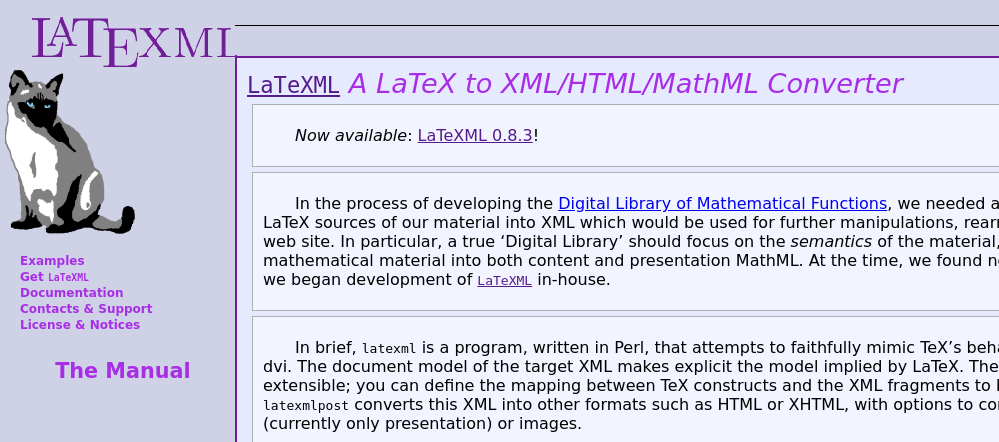
\includegraphics[width=0.9\textwidth]{ltxml_website.png}
    
\includegraphics[width=0.9\textwidth]{ltxml_github2.png}
    
\includegraphics[width=0.9\textwidth]{ltxml_github1.png}
    \begin{flushright}
        {\tiny credit: Bruce Miller, \texttt{www.nist.gov/people/bruce-r-miller}}
    \end{flushright}
\end{frame}

%%%%FRAME
\begin{frame}{Obtaining and Classifying Definitions}
    \begin{itemize}
        \item Sometimes the author of an article uses a \LaTeX{} macro to label a definition. These are our positive labels:
    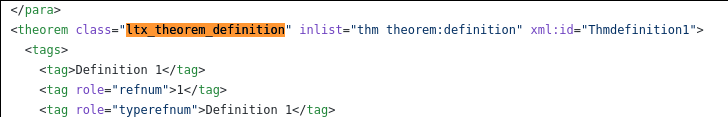
\includegraphics[width=0.9\textwidth]{ltxml_defin_xml.png}
    \item To get negative labels, we pick paragraphs at random and assume they are not definitions.
        \item This has the drawback that some of the non--definitions are wrong.
    \item There are 1,707 articles in 2015 math.AG, we go from 5,229 labeled definitions to 71,067 ``probable'' definitions.  \end{itemize}
\end{frame}


%%%%FRAME
\begin{frame}{Some Classification Results}
    \begin{itemize}
        \item Results using SVC (Support Vector Classifier) in \textbf{scikit-learn}
    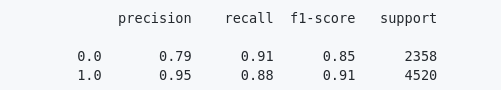
\includegraphics[width=0.7\textwidth]{class_results_svc.png}
    \item Sanity check:
    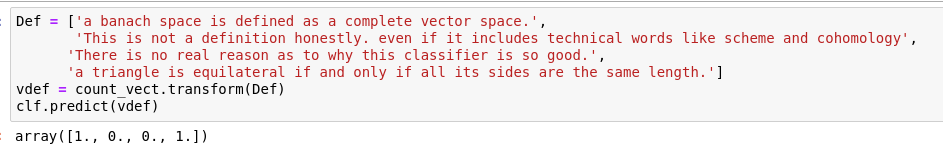
\includegraphics[width=0.95\textwidth]{sanity_check.png}
    \end{itemize}
    \begin{center}
     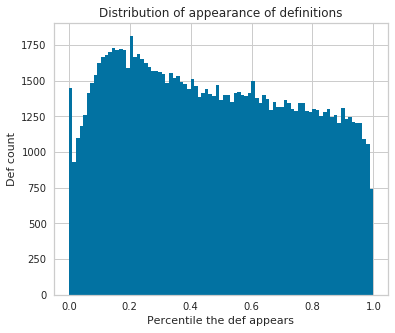
\includegraphics[width=0.5\textwidth]{def_appear_hist.png}
    \end{center}
\end{frame}

%%%%FRAME
\begin{frame}{Extracting the Definienda}
    \framesubtitle{Obtaining the data for Named Entity Recognition system}
    \begin{columns}[T]
        \begin{column}{0.5\textwidth}
    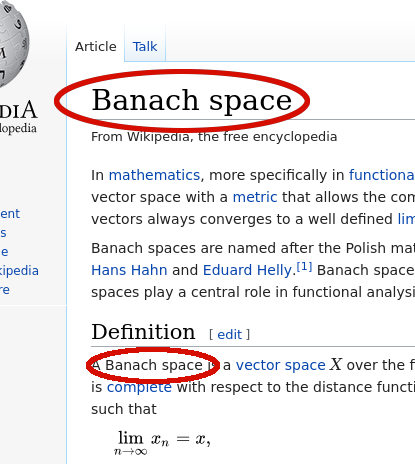
\includegraphics[width=\textwidth]{wiki_thin_banach.png}
        \end{column}
        \begin{column}{0.5\textwidth}
            \begin{itemize}
            \item Go through every of wikipedia article looking for a Definition section that contains the title.
            \item We obtain a pair:\\
                (\textbf{Definienda},  Definition).
            \item Just 5,321 matches out of almost 6 million articles.
            \item Several other websites could be used e.g. The Stacks project
            \end{itemize}
        \end{column}
    \end{columns}
\end{frame}

%%%%FRAME
\begin{frame}{Training and Evaluating the NER System} 
    \framesubtitle{Results of the IOB parser using the ChunkParserI method in the \textbf{nltk} library}
    \begin{columns}[T]
        \begin{column}{0.5\textwidth}
            \begin{tabular}{|c|c|r|}
                \hline
                \hline
        \multicolumn{2}{|c|}{\color{blue}{Input}} & \color{purple}{Output} \\
                \hline
                \hline
                \color{blue}{Token} & \color{blue}{POS} & \color{purple}{NER}\\
                \hline
                  We&PRP&O\\
                  \hline
                  define&VBP&O\\
                  \hline
                  a&DT&O\\
                  \hline
                  Banach&NNP&B--DFNDUM\\
                  \hline
                  space&NN&I--DFNDUM\\
                  \hline
                  as&IN&O\\
                  \hline
                  a&DT&O\\
                  \hline
                  complete&JJ&O\\
                  \hline
                  vector&NN&O\\
                  \hline
                  space&NN&O\\
                  \hline
            \end{tabular}
    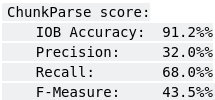
\includegraphics[width=0.6\textwidth]{BIO_stats.png}
        \end{column}
        \begin{column}{0.5\textwidth}
            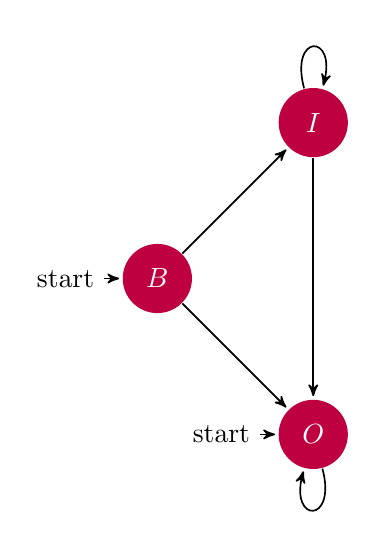
\begin{tikzpicture}[scale=0.5, ->,>=stealth',shorten >=1pt,auto,node distance=2.8cm, semithick ]
  \tikzstyle{every state}=[fill=purple,draw=none,text=white]

  \node[initial,state] (A)                    {$B$};
  \node[state]         (B) [above right of=A] {$I$};
  %\node[state]         (D) [below right of=A] {$q_d$};
  \node[initial,state]         (C) [below right of=A] {$O$};
  %\node[state]         (E) [below of=D]       {$q_e$};

  \path (A) edge              node {} (B)
            edge              node {} (C)
        (B) edge [loop above] node {} (B)
            edge              node {} (C)
        (C) edge [loop below]  node {} (C);
\end{tikzpicture}

        \end{column}
    \end{columns}
\end{frame}

%%%%FRAME
\begin{frame} 
    Some definitions found in the 2015 math.DG articles:
    \begin{block}{Ex. Things we like}
        {\small An {\color{blue}induced generalized Kähler structure} on \_inline\_math\_ is a Lie algebraic generalized Kähler structure with \_inline\_math\_. It is a canonical generalized Kähler structure if \_inline\_math\_.}
    \end{block}
    \begin{exampleblock}{Ex. Things we don't like}
        {\small Suppose \_inline\_math\_ is a {\color{darkgreen}vector space}. The only connection on the {\color{darkgreen}graded manifold} \_inline\_math\_ is the {\color{blue}trivial connection}.}
    \end{exampleblock}
        \begin{center}
    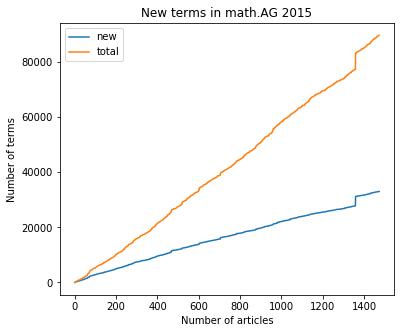
\includegraphics[width=0.5\textwidth]{cum_terms.png} 
        \end{center}
\end{frame}
%%%%FRAME
\begin{frame} 
    \frametitle{Conclusions and Future Work}
    \begin{itemize}
            \item We think that we have collected enough evidence to believe that a robust collector of definitions is possible.
            \item A lot of interesting work ahead:
                \begin{itemize}
                    \item Organize the definitions in a \emph{dependency tree structure.}
                    \item Produce word embedding with math tokens\\
                        (e.g. where \emph{Banach space} is just one token).
                \item Visualize the new terminology to assist with classification and disambiguation. 
                \end{itemize}
    \end{itemize}
\end{frame}

%%FRAME
\begin{frame}
\titlepage
\end{frame}


\end{document}

% I removed this table to have a cleaner format
%    {\tiny\begin{tabular}{|l|l|}
%        \hline
%        almost flat manifold  &   An almost flat manifold whose 2-sylow subgroup of the holonomy group...\\
%        \hline
%        An infranilmanifold  &   An infranilmanifold is a double coset space \_inline\_math\_ where \_inli...\\
%        \hline
%        normal subgroup  &   Let \_inline\_math\_. Then \_inline\_math\_ is a normal subgroup of \_inline...\\
%        \hline
%        central involution  &   A central involution \_inline\_math\_ of an infranilmanifold \_inline\_mat...\\
%        \hline
%        infranilmanifold  &   Any infranilmanifold \_inline\_math\_ with \_inline\_math\_ a 2-group has a...\\
%        \hline
%        vector bundle  &   A vector bundle \_inline\_math\_ is flat if it has finite structure grou...\\
%        \hline
%        Tangent bundles of  &   Tangent bundles of infranilmanifolds are flat:...\\
%        \hline
%        warped product  &   The warped product provides a way to construct new pseudo-riemannian...\\
%        \hline
%        Dualistic structures  &   Dualistic structures are closely related to statistical mathematics....\\
%        \hline
%        affine connection  &   In the notions of terms on statistical manifolds, for a torsion-free...\\
%        \hline
%        horizontal lift  &   Let \_inline\_math\_ in \_inline\_math\_. The horizontal lift of \_inline\_ma...\\
%        \hline
%    \end{tabular}}
